% \subsection{Packet Steering Offload}
\noindent  {\textbf{Packet Steering Offload.}} We begin by evaluating the impact of packet steering to programmable NICs, and compare a pure software-based UPF (\S\ref{sub:swUPF}) with a UPF that offloads packet steering to programmable hardware (\S\ref{sub:steerOffload}). Figure~\ref{fig:AvsB_tput} shows the throughput and latency of both the designs when we dedicate $2$ cores for dataplane processing---one for uplink traffic and another for downlink traffic. As expected, we find that offloading packet steering leads to $45 \%$ higher throughput and up to $37 \%$ lower latency (except when both designs saturate linerate at maximum packet size), due to lesser overhead of intercore communication and packet steering in the offloaded design. However, the performance gains due to this offload also come with a loss in flexibility. We consider a scenario where a UPF has to dynamically scale the number of cores it is running on due to an increase in incoming traffic. Figure~\ref{fig:AvsB_dyn_scl} shows the UPF throughput during scaleup, and we see the adverse impact of having to restart the port and reconfigure hardware queues in the offload design. Next, we configure our RAN emulator in such a way that 20\% of the UEs processed by a single worker core generate a sudden burst of traffic, and Figure~\ref{fig:AvsB_rebal} shows how the offload design suffers high latency due to its inability to balance load across cores in the presence of such ``heavy-hitter'' UEs. {\em In summary, we find that offloading packet steering to NICs leads to significant performance gains, but comes at a loss of flexibility that can hurt operators that expect to perform dynamic scaling frequently or see skewed traffic across users. }
%Note that both the designs are scalable across cores. SoftUPF takes $3$ and $4$ cores to saturate $40G$ linerate in the uplink and downlink respectively. In contrast, the SteerOffload design takes $2$ and $3$ cores to saturate uplink and downlink respectively. 
%deally, the latency after rebalancing should be same as when there was less load. But we observe that there is a slight increase in the heavy hitter latency. We have also noticed that this latency after rebalancing further increases if the load from heavy hitter UEs is increased further. This is because we have used a very simple rebalancing algorithm which is sub-optimal. We expect that an optimal algorithm with a better heuristic will prevent/reduce this increase in latency, and consider it as one of our future works. However, even with this sub-optimal algorithm and increase in latency, we see that this is still less than the RTT latency for a heavy hitter in the RTC design.
% \begin{figure}[t]
% \centering
%   \begin{tabular}{@{}cc@{}}
%     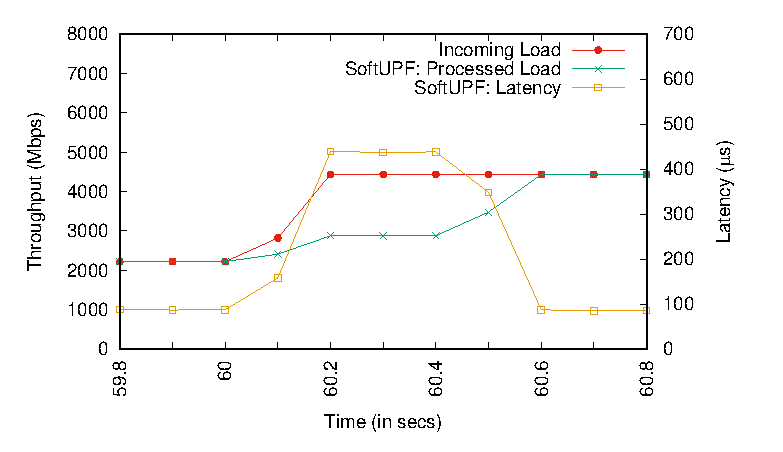
\includegraphics[width=.25\textwidth]{graphs/dynScaling_softUPF} &
%     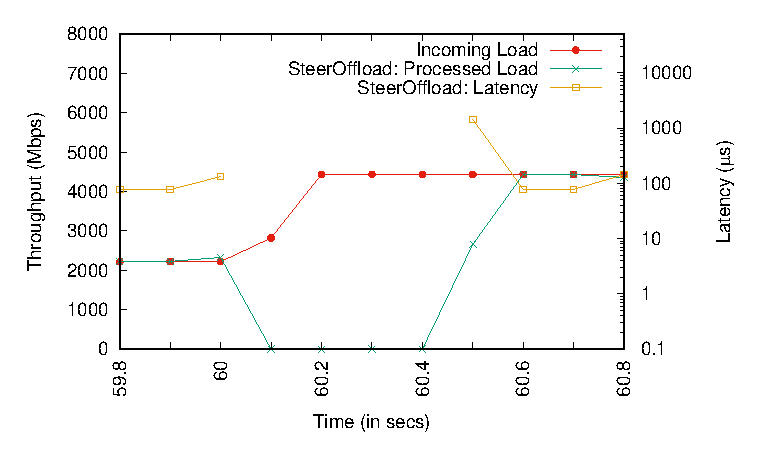
\includegraphics[width=.25\textwidth]{graphs/dynScaling_SteerOffload}    \\
%   \end{tabular}
%    \caption{SoftUPF vs SteerOffload: Dynamic Scaling.}
%  \label{fig:AvsB_dyn_scl}
% \end{figure}

% \begin{figure}[t]
%  \centering
% 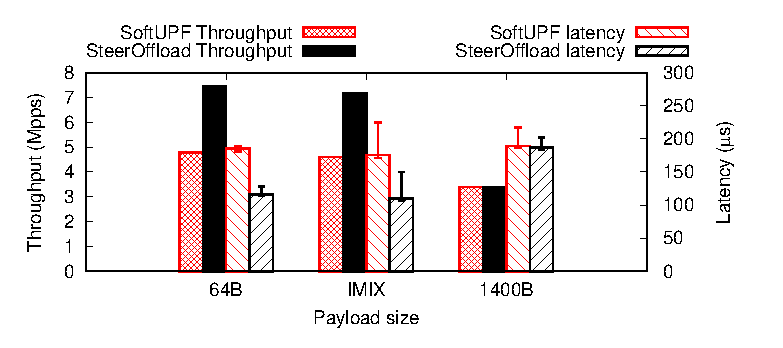
\includegraphics[width=0.45\textwidth]{graphs/pipelineVsRTT}
%  \setlength{\abovecaptionskip}{4pt}
%  \setlength{\belowcaptionskip}{-12pt}
%  \caption{SoftUPF vs. SteerOffload: Performance.}
%  \label{fig:AvsB_tput}
% \end{figure}
% 
% \begin{figure}[t]
%     \centering
%      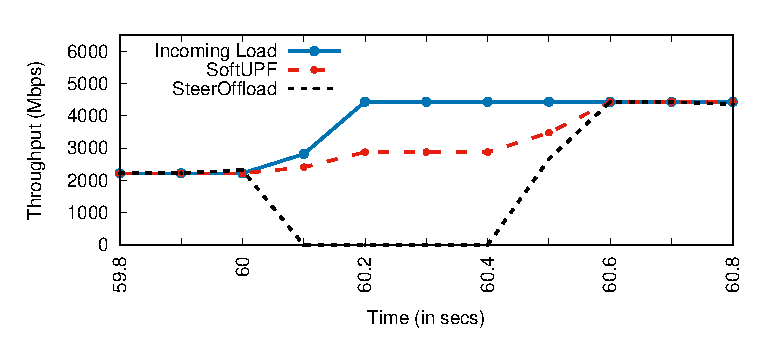
\includegraphics[width=0.4\textwidth]{graphs/dynScaling} % second figure itself
%      \setlength{\abovecaptionskip}{4pt}
%      \setlength{\belowcaptionskip}{-8pt}
%  \caption{SoftUPF vs. SteerOffload: Dynamic Scaling.}
% %  \caption{Dynamic Scaling.}
%  \label{fig:AvsB_dyn_scl}
% \end{figure}
% 
% % \begin{figure}[t]
% %     \centering
% %     \begin{minipage}{0.235\textwidth}
% %         \centering
% %         \subfloat[SoftUPF]{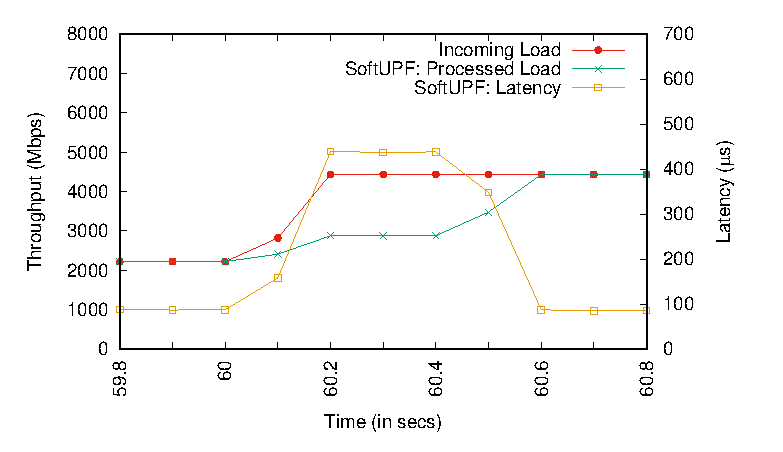
\includegraphics[width=\textwidth]{graphs/dynScaling_softUPF}} % first figure itself
% %     \end{minipage}
% % \hfill
% %     \begin{minipage}{0.235\textwidth}
% %         \centering
% %          \subfloat[SteerOffload]{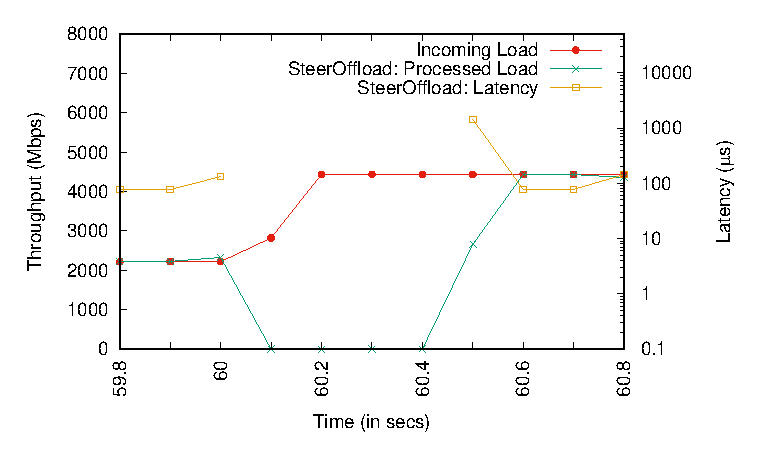
\includegraphics[width=0.99\textwidth]{graphs/dynScaling_SteerOffload}} % second figure itself
% %     \end{minipage}
% %      \setlength{\abovecaptionskip}{4pt}
% %      \setlength{\belowcaptionskip}{-12pt}
% %  \caption{SoftUPF vs SteerOffload: Dynamic Scaling.}
% %  \label{fig:AvsB_dyn_scl}
% % \end{figure}
% 
% \begin{figure}[t]
%  \centering
% 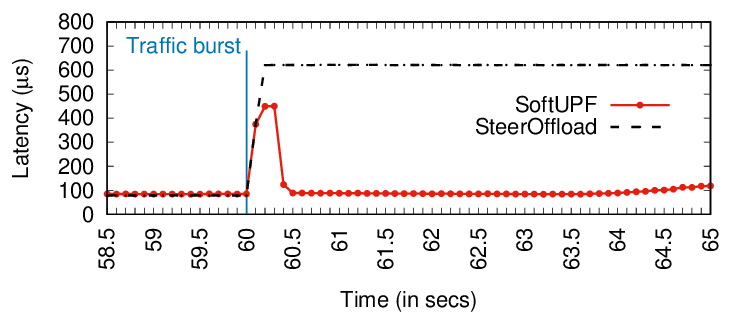
\includegraphics[width=0.4\textwidth]{graphs/heavyHitter}
%  \setlength{\abovecaptionskip}{4pt}
%  \setlength{\belowcaptionskip}{-8pt}
%   \caption{SoftUPF vs. SteerOffload: Heavy hitters.}
% %  \caption{SoftUPF vs SteerOffload: Heavy hitter redistribution.}
%  \label{fig:AvsB_rebal}
% \end{figure}

% XXX: can combine throughput and latency in one graph with two y-axis, when showing results for different scenarios.

% XXX: Are throughput results for single core?

% XXX: need a graph to show throughput as a function of number of cores. This is only place where we show DPDK UPF hitting linerate. Or at least mention in the text that performance scales with cores and we can saturate linerate at XXX cores.  

% XXX: Keep the dynamic scaling and heavy hitter graphs simple, with one load change/scaling event. Do not clutter with datapoints.
